\documentclass[10pt,A4,makeidx]{article}
\usepackage{graphicx}
\usepackage{grffile}
\usepackage{color}
\usepackage{amsmath}
\usepackage{float}
\usepackage{subfig}
\usepackage{comment}
\UseRawInputEncoding

\graphicspath{ {./visuals/} }

\textwidth 18cm
\hoffset -3.0cm
\textheight 24cm
\voffset -2.5cm

\newcommand{\tR}{\texttt{R}}
\newcommand{\adist}{\overset{\cdot}{\underset{\cdot}{\sim}}}
%\setcounter{tocdepth}{2}

\title
{Effects of Structural Characteristics on House Prices}
\author{Sean Peralta Garcia (23088091)}
\date {}

\usepackage{Sweave}
\begin{document}

\maketitle


\section{Executive Summary}
  Important aspects of the model - logarithmic
  Important terms
  Final Model\\
  This report aims to investigate the variables that influence house prices.
  The variables available for analysis include, house size, number of bedrooms,
  number of bathrooms, land size, age and presence of a fireplace. It was concluded that
  the main variables that influence house prices were, house size and its number of bathrooms;
  the age and presence of a fireplace were also used in obtaining an accurate prediction
  of house prices. This can be modelled through the equation:
  
  \begin{center}
    \textbf{    \(\ln Price = \beta _0 + \beta _1 Size + \beta _2 Baths + \beta _3 Fireplace + \beta _4 \log_{10}Age + \varepsilon\)\\}
  \end{center}

\section{Introduction}
  Owning a house is one of the biggest investments a person can make. As such, it 
  is of great interest to prospective buyers, sellers and lenders to accurately
  predict the price of a home. There are a range of models and techniques that 
  attempt to predict the price of a home, from observational appraisals all 
  the way to machine learning models[2]. One method widely studied is that of
  hedonic pricing. A Hedonic Pricing Model (henceforth, HPM) is a model that 
  attempts to estimate the price of a good by taking its observable characteristics
  and then weighting them according to their relative impact on the price. Models
  utilise a range of measures that can be categorised into several groups, 
  namely structural, neighbourhood, and environmental.[3] Hearth and Maier,
  in a literature review of HPMs for real estate, had identified that the 
  neighbourhood and environmental factors were generally over-researched. While
  social factors and the "implicit value of structural characteristics" was 
  under-researched.[1]

  \subsection{Related Work}
  There appears to be a consensus that creating a HPM, particularly focussing on
  structural characteristics, has problems with heteroskedasticity. This means
  that linear models may not be entirely appropriate to estimate the response.
  This was sought to be relieved by Selim, Limsombunchai and Malpezzi by using
  a semi-logarithmic form wherein the response variable is transformed by the natural log.[2, 3, 4]
  Additionally, Malpezzi explains
  that this effectively allows value added to the house to be proportional to 
  other variables in the model and for an easier interpretation of coefficients
  such that the coefficient of a measure is the percentage change for 1 unit 
  difference in the measure.[3]
  In the end Selim concluded that water system, presence of a pool, the type of house,
  number of rooms, house size, locational characteristics and building type were
  the most significant variables to affect house prices in the country of Turkey.[4]
    
  \subsection{Data Set}
  The data set contains data on houses in Saratoga County, New York; collected by
  Candice Corvetti in 2006. It contains 1063 randomly selected observations collecting
  data on house price, size in square feet, number of bathrooms, number of bedrooms,
  the presence of a fireplace, land size in acres and the age of the house in years.
  
  \subsection{Aim}
  The aim of this report is to fit a model that will attempt to determine how 
  the price of a house depends its structural characteristics. Significant 
  variables that appear in the Turkish model will be explored in the Saratoga 
  data set to see if they also play a significant role in predicting house price.

\section{Methodology}
The methodology to be used in this report will be split into two parts. Data
exploration and model fitting.
  \subsection{Data Exploration}
  Firstly, the scatter plots between independent and dependent variables will be 
  visually analysed to identify relationships and distribution of data. Strangely
  distributed data will attemp to be transformed to find a linear relationship to 
  the price. After, scatter plots between independent variables will be visually analysed to quickly 
  identify multicollinear variables. Additionally, correlation analysis will be used to 
  supplement the visual analyses. This process will aim to identify redundant and 
  non-contributing variables that we may expect will be excluded from the 
  final model.  
  Variables that are suspected to have interaction are investigated by running linear 
  regressions with only those interaction terms and analysing the interaction plots.
  If an interaction effect is apparent then that interaction term will be considered
  in model fitting.
  \subsection{Model fitting}
  Model fitting will be done with backwards elimination, including found interaction 
  variables. Then, the collinear and redundant variables will be removed from the 
  model and tested using the F-test to check for a better fit. Then normal backwards elimination, in which 
  where variables eliminated from the model if they have a low significance to the model, is applied.
\section{Results}
  \subsection{Data Exploration}

  Below are the relationships between the Price and independent variables.\\
  \emph{Correlation data in appendix figure 1 and 2.}
  \begin{itemize}
    \item Size - exhibits a strong, positive linear relationship. (correlation: 0.77)
    \item Baths - exhibits a moderate, positive linear relationship. (correlation: 0.67)
    \item Bedrooms - exhibits a moderate linear relationship (correlation: 0.47)
    \item Fireplace - exhibits a weak, positive linear relationship - houses 
    with a fireplace have a higher range of price, as well as a higher mean (correlation: 0.41)
    (\emph{Correlation data in appendix figure 3.})
    \item Acres - little to no linear relationship - data is heavily right skewed 
      \subitem - acres are all clustered closer to 0 (correlation: 0.18)
    \item Age - little to no linear relationship - heavily right skewed
      \subitem - majority of properties are grouped
    towards 0 age (correlation: -0.26)\\
  \end{itemize}
  
  Acres and age appeared to show a right skewed nature, therefore a logarithmic transformation was applied
  in order to achieve a more normal distribution.\emph{Figure 4 - Correlation coefficients for log transformed data}\\
  
  \emph{Price by Acres and Price by Age}\\
  \begin{center}
    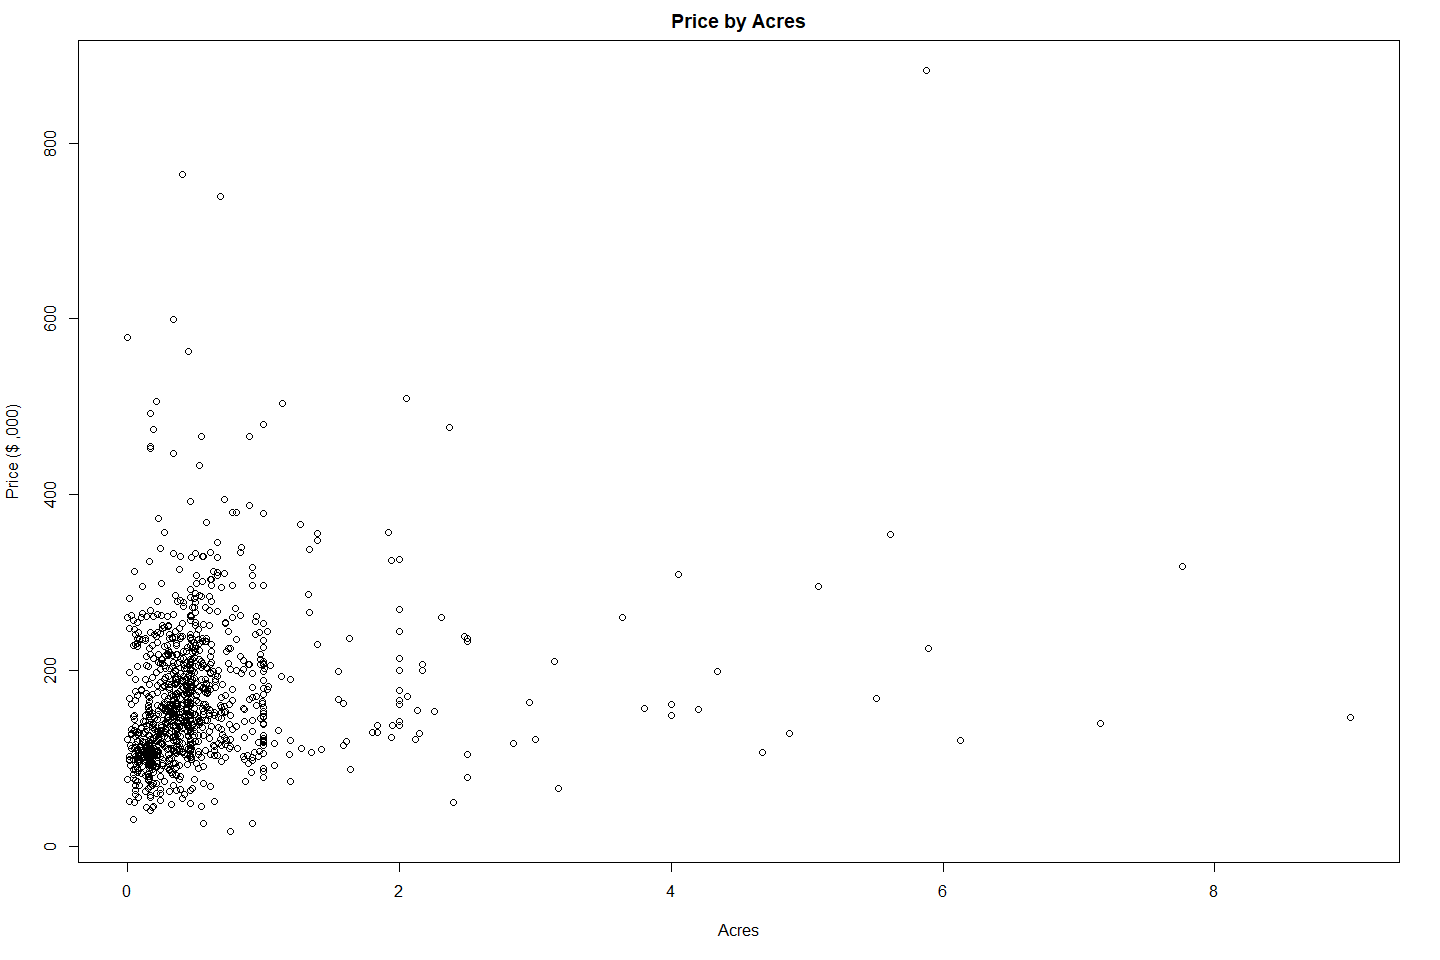
\includegraphics[width=8cm]{price-acres.png}
    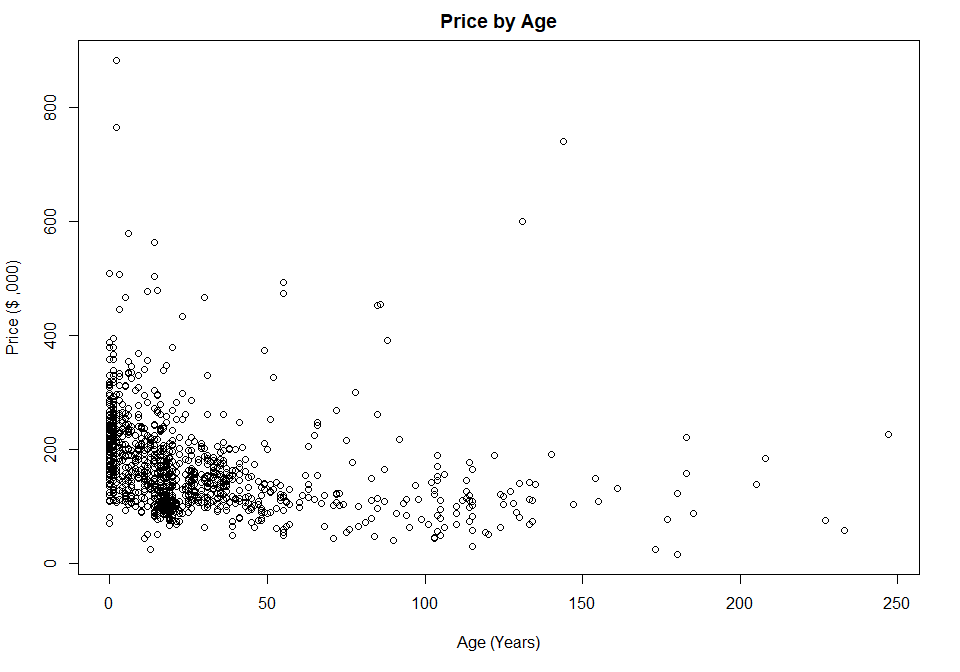
\includegraphics[width=8cm]{price-age.png}
  \end{center}
  
  \emph{Price by log10(Acres) and Price by log10(Age)}\\
  \begin{center}
    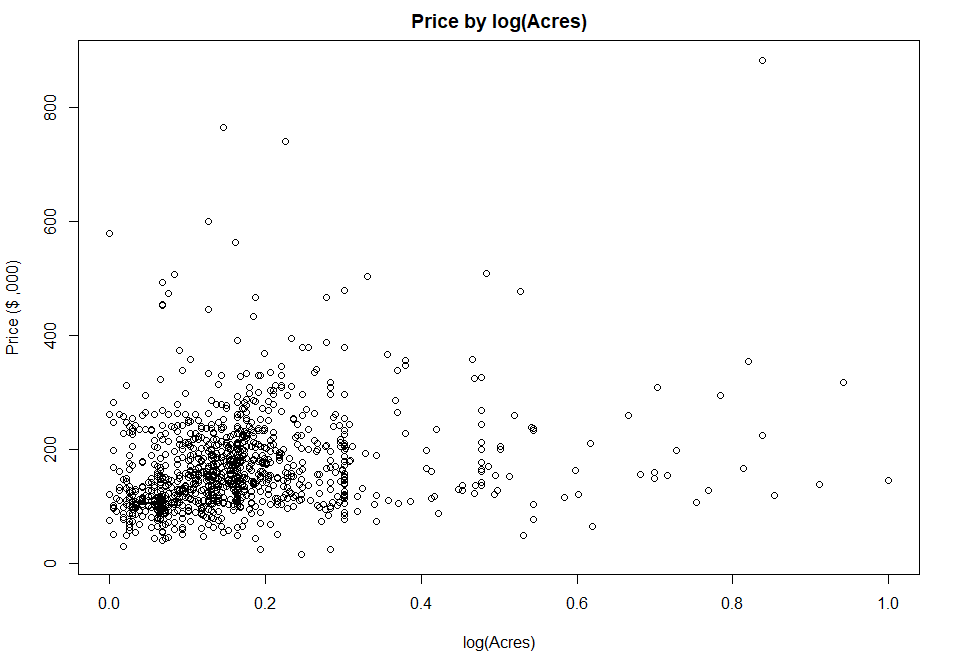
\includegraphics[width=8cm]{price-logacres.png}
    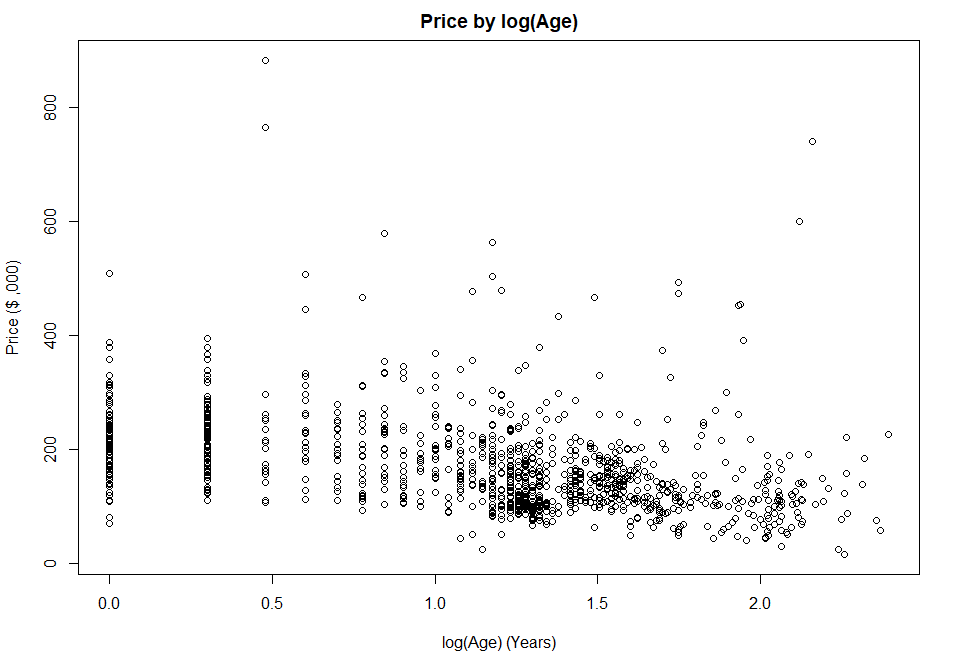
\includegraphics[width=8cm]{price-logage.png}
  \end{center}
  
  Now we will find collinear variables, firstly by visually inspecting the plot
  of all variables (\emph{see appendix fig. 2}). From this we can observe that the
  following have correlations of:
  \begin{itemize}
    \item Size and Baths (correlation: 0.77)
    \item Size and Bedrooms (correlation: 0.67)
    \item Baths and Bedrooms (correlation: 0.51)
  \end{itemize}
  
  Interaction terms involving the fireplace metric were investigated as it was the only 
  categorical variable available to us. Only the size variable appeared to
  have somewhat of an interaction as shown below. Black dots showing no fireplace, and
  red dots showing the presence of a fireplace. Fireplaces seem to appear in houses 
  of all sizes but as houses become larger, the more prevalent a fireplace becomes An
  analysis of variance on this interaction returns a p-value of p=3.19e-10.\\
  \begin{center}
    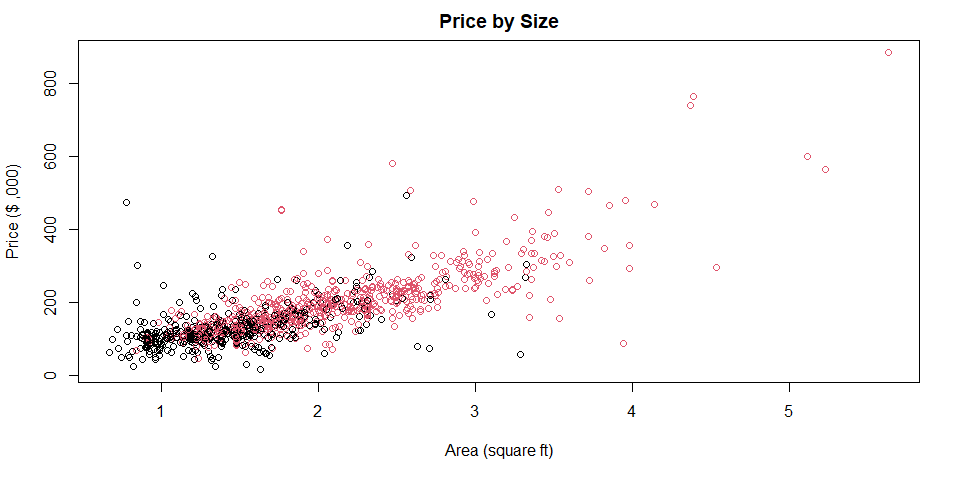
\includegraphics[width=15cm]{int-fireplacesize.png}
  \end{center}

  \subsection{Model fitting}
  \begin{center}
    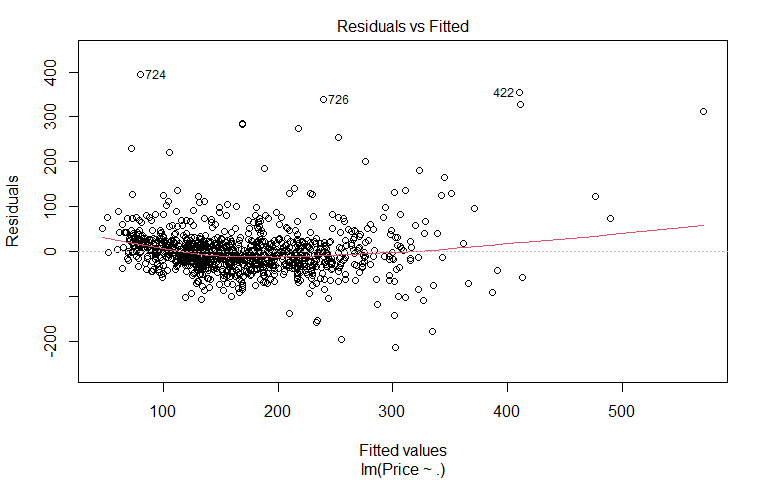
\includegraphics[width=8cm]{full-res.png}
    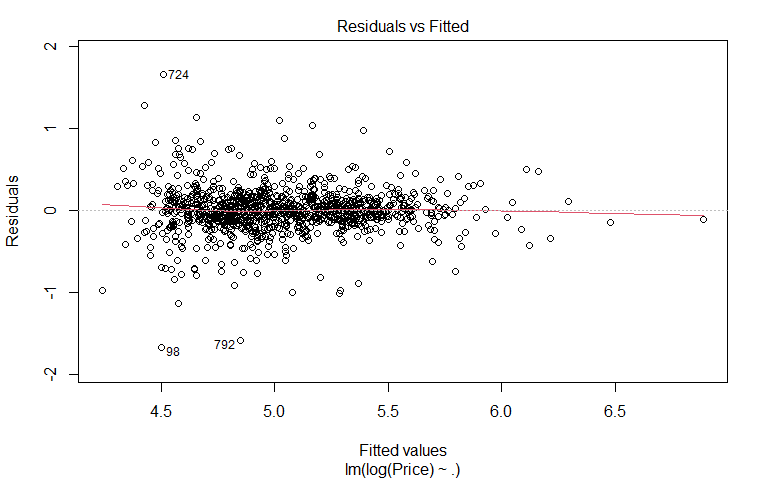
\includegraphics[width=8cm]{full-resln.png}
  \end{center}
  First fitted the full model (without interactions) was fitted, without the interaction. And the residuals were plotted.
  The errors to the fitted line were not constant and this was reflected in the high Residual Standard Error
  (52.15), thus confirming the presence of heteroskedasticity described in the literature.
  As suggested by previous studies, I applied a natural log function to the response variable.
  This model returned a much lower RSE of 0.279, thus indicating the response variable
  much closely follows a log relationship to the independent variables in the model.

  Next, the  starting model(with interactions) for is given by the formula:\\

  \(\ln Price = \beta _0 + \beta _1 Size + \beta _2 Baths + \beta _3 Bedrooms + \beta _4 Fireplace + \beta _5 \log_{10}Acres + \beta _6 \log_{10}Age + \beta _7 Fireplace*Size + \varepsilon\)\\

  Through backwards elimination, the variables of bedrooms, fireplace, acres and
  fireplace \& size interaction are eliminated. thus the final model is:\\
  
  \(\ln Price = \beta _0 + \beta _1 Size + \beta _2 Baths + \beta _3 Fireplace + \beta _4 \log_{10}Age + \varepsilon\)\\
  
  The final model has an RSE of 0.2819, and adjusted R-squared of 0.6087 and a
  F-statistic of 414.\\

\section{Discussion}
  Due to the low correlations of fireplace we can assume that it is likely to be
  a non-contributing variable and unlikely to come up in the final model\\
  

  age and acres might have been able to be transformed in order to find a relationship - not really\\

  Due to the multicollinearity shown by size, baths and bedrooms variables, we will
  likely exclude one or two of these variables from the final model. The variable
  with the highest correlation to the price is Size. Therefore Baths and Bedrooms
  may end up exluded in the final model. \\
  
  At this point, the data would have pointed to removing all but the size variable from the model.\\
  
  perhaps a more thorough data exploration with more interaction terms + interaction terms with continuous vars in bins + interaction chosen may not have been overly relevant?
  and more in depth visualisations would aide in the creation of the final model.\\
  
  Final Model - 

\bibliographystyle{apalike}
\begin{thebibliography}{9}
\bibitem{lit_rev}
Herath, S. K. Maier, G. (2010). The hedonic price method in real estate and housing market research. A review of the literature.. Institute for Regional Development and Environment (pp. 1-21). Vienna, Austria: University of Economics and Business.

\bibitem{hedonic_ai}
Limsombunchai, V. (2004). House price prediction: Hedonic price model vs. artificial neural network. New Zealand Agricultural and Resource Economics Society Conference, 25-26 June 2004. Blenheim, New Zealand: New Zealand Agricultural and Resource Economics Society.

\bibitem{hedonic_rev}
Malpezzi, S. (2003). Hedonic pricing models: a selective and applied review. Housing economics and public policy, 1, 67-89.

\bibitem{hedonic_regress}
Selim, S. (2008). DETERMINANTS OF HOUSE PRICES IN TURKEY: A HEDONIC REGRESSION MODEL . Dogus Universitesi Dergisi , 9 (1) , 65-76 . Retrieved from 
\end{thebibliography}

\pagebreak
\section*{Appendix.}
  \emph{\\Figure 1 - Correlation coefficients for untransformed data}
  \begin{Soutput}
              Price  Size Baths Bedrooms Fireplace Acres   Age
    Price      1.00  0.77  0.67     0.47      0.41  0.18 -0.26
    Size       0.77  1.00  0.74     0.67      0.47  0.22 -0.23
    Baths      0.67  0.74  1.00     0.51      0.45  0.13 -0.40
    Bedrooms   0.47  0.67  0.51     1.00      0.30  0.15 -0.04
    Fireplace  0.41  0.47  0.45     0.30      1.00  0.06 -0.24
    Acres      0.18  0.22  0.13     0.15      0.06  1.00  0.01
    Age       -0.26 -0.23 -0.40    -0.04     -0.24  0.01  1.00
  \end{Soutput}
  
  \emph{Figure 2 - All plots}\\
  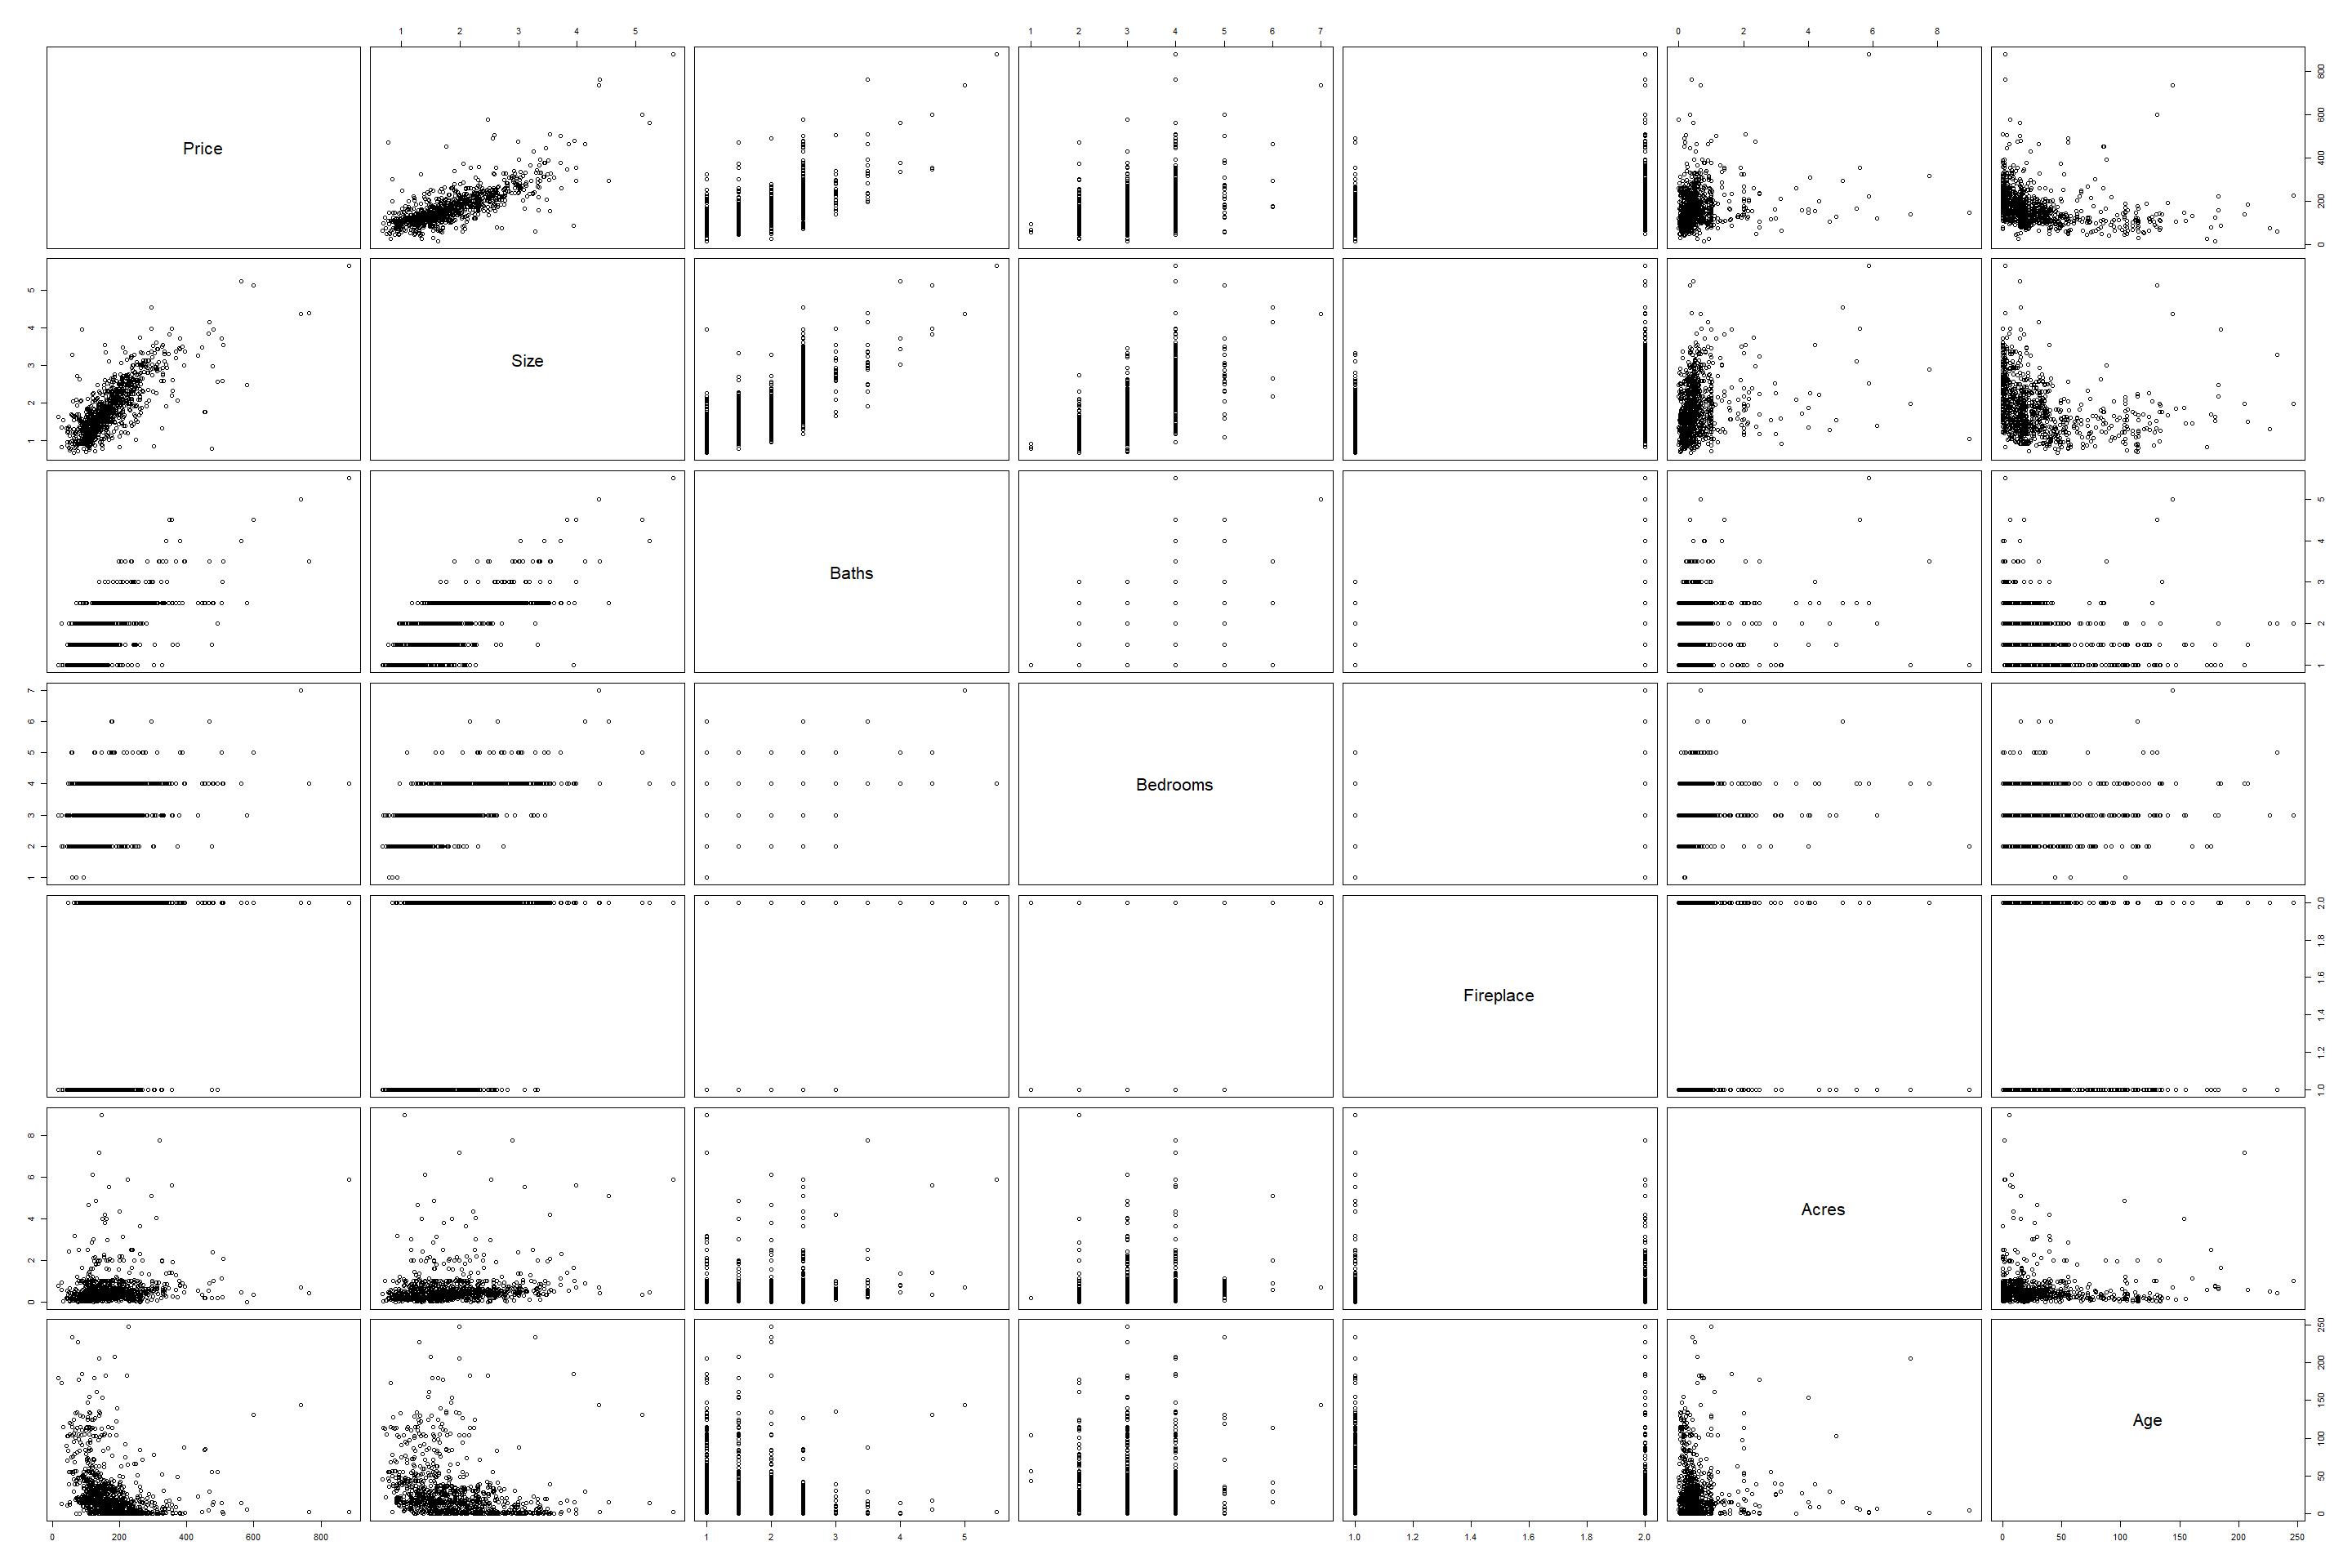
\includegraphics[scale=2]{plot.png}
  
  \emph{Figure 3 - Price by Fireplace boxplot}\\
  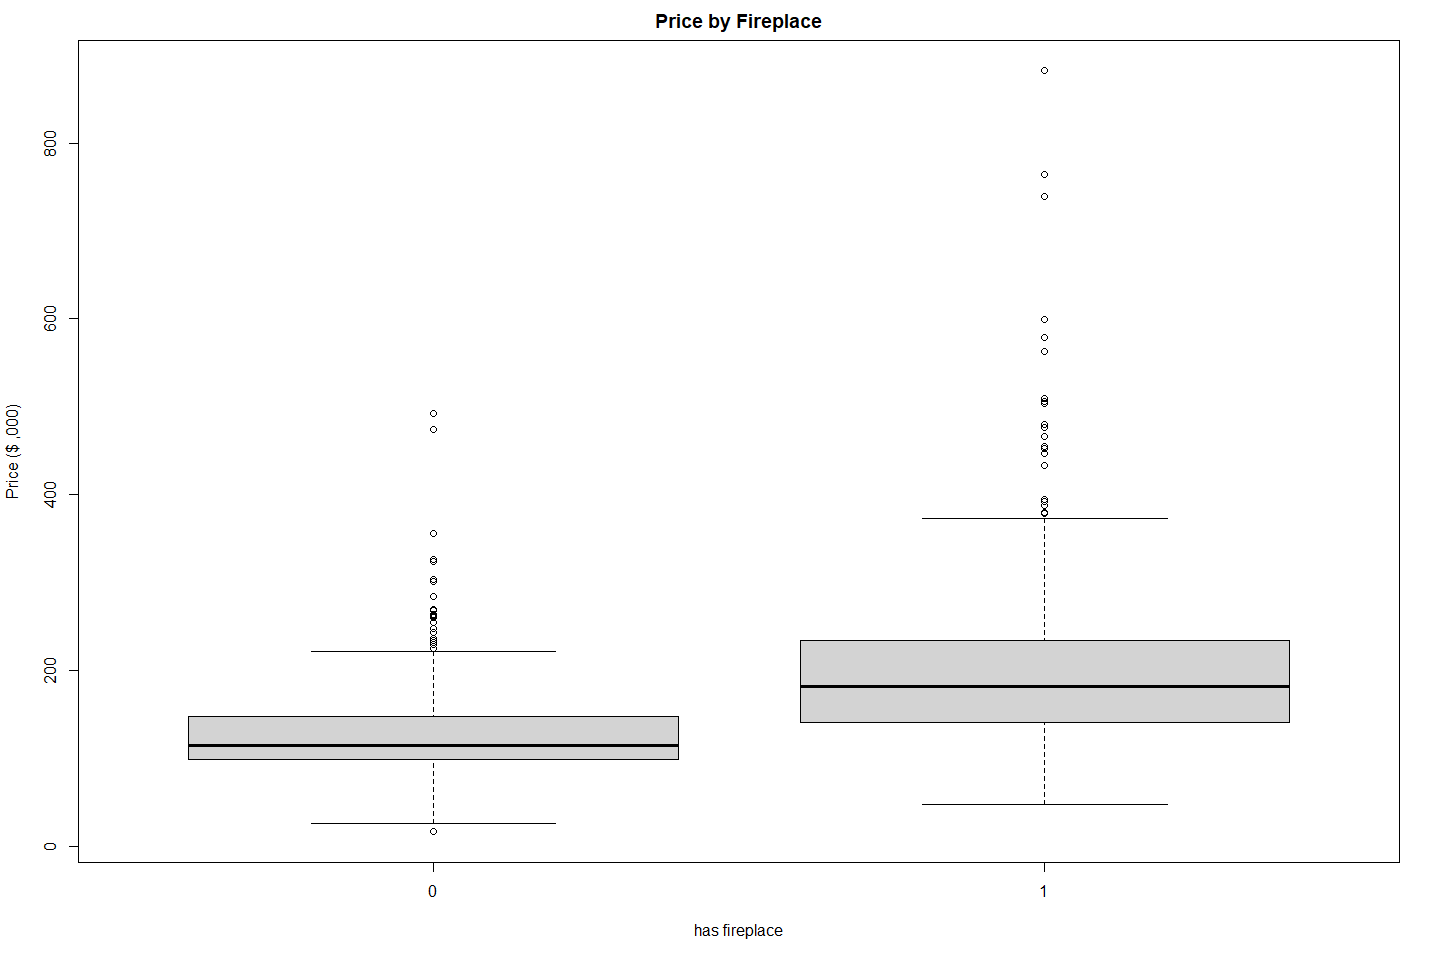
\includegraphics[scale=0.4]{price-fireplace.png}
  
  \emph{\\Figure 4 - Correlation coefficients for log transformed data}
  \begin{Soutput}
              Price  Size Baths Bedrooms Fireplace Acres   Age
    Price      1.00  0.77  0.67     0.47      0.41  0.22 -0.39
    Size       0.77  1.00  0.74     0.67      0.47  0.28 -0.42
    Baths      0.67  0.74  1.00     0.51      0.45  0.17 -0.53
    Bedrooms   0.47  0.67  0.51     1.00      0.30  0.22 -0.18
    Fireplace  0.41  0.47  0.45     0.30      1.00  0.12 -0.29
    Acres      0.22  0.28  0.17     0.22      0.12  1.00 -0.08
    Age       -0.39 -0.42 -0.53    -0.18     -0.29 -0.08  1.00
  \end{Soutput}
  
  \emph{\\Figure 5 - Full model + Fireplace:Size Statistics\\}
  $\ln Price = \beta _0 + \beta _1 Size + \beta _2 Baths + \beta _3 Bedrooms + \beta _4 Fireplace + \beta _5 \log_{10}Acres + \beta _6 \log_{10}Age + \beta _7 Fireplace*Size + \varepsilon$
  \begin{Soutput}
    Residual standard error: 0.282 on 1055 degrees of freedom
    Multiple R-squared:  0.611,	Adjusted R-squared:  0.6084 
    F-statistic: 236.7 on 7 and 1055 DF,  p-value: < 2.2e-16
  \end{Soutput}

  \emph{\\Figure 6 - Final model Statistics\\}
  $\ln Price = \beta _0 + \beta _1 Size + \beta _2 Baths + \beta _3 Fireplace + \beta _4 \log_{10}Age + \varepsilon$
  \begin{Soutput}
    Residual standard error: 0.2819 on 1058 degrees of freedom
    Multiple R-squared:  0.6101,	Adjusted R-squared:  0.6087 
    F-statistic:   414 on 4 and 1058 DF,  p-value: < 2.2e-16
  \end{Soutput}
  
  \emph{\\Figure 6 - Final model Statistics\\}
  $\ln Price = \beta _0 + \beta _1 Size + \beta _3 Baths + \beta _5 Fireplace + \beta _7 \log_{10}Age + \varepsilon$
  \begin{Soutput}
Coefficients:
             Estimate Std. Error t value Pr(>|t|)    
(Intercept)   4.23022    0.04591  92.134  < 2e-16 ***
Size          0.31402    0.01933  16.247  < 2e-16 ***
Baths         0.13768    0.02097   6.564 8.19e-11 ***
FireplaceYes  0.11638    0.02031   5.729 1.32e-08 ***
Age          -0.09263    0.01791  -5.172 2.77e-07 ***
  \end{Soutput}


\end{document}
